\RequirePackage[dep]{snapshot}
\documentclass{econtex}\usepackage[pdftex]{graphicx}\usepackage{epstopdf} \usepackage[pdftex]{hyperref}
\usepackage{moreverb}
%\usepackage{fourier} \usepackage[scaled=0.87]{berasans} \usepackage[scaled=0.87]{beramono}

\usepackage{amsmath,graphicx,url,rotating,dcolumn,booktabs,natbib,authblk,verbatim}
\usepackage{floatpag}
\usepackage{subfigure,cancel,amsfonts,amssymb,bbm}
%\usepackage{geometry}

\usepackage[marginparwidth=0in,left=1.65in,right=1.65in,top=1.65in,bottom=1.65in]{geometry}

%\usepackage[mathcal]{eucal}
\usepackage{threeparttable}
%\usepackage[nolists]{endfloat}

\newcommand{\N}{\mathbb{N}}
            \newcommand{\R}{\mathbb{R}}
            \newcommand{\aboveMin}{\blacktriangle}
            \newcommand{\aAgg}{\ensuremath{\mathsf{A}}}
            \newcommand{\adj}{\ensuremath{\mathrm{j}}}
            \newcommand{\adjPar}{\ensuremath{\omega}}
            \newcommand{\aE}{\aRat^{e}}
            \newcommand{\aFunc}{\ensuremath{\mathrm{a}}}
            \newcommand{\Age}{\ensuremath{Z}}
            \newcommand{\age}{\ensuremath{z}}
            \newcommand{\ALevBF}{\ensuremath{\mathbf{A}}}
            \newcommand{\aLevBF}{\ensuremath{\mathbf{a}}}
            \newcommand{\ALev}{\ensuremath{\pmb{A}}}
            \newcommand{\aLev}{\ensuremath{\pmb{a}}}
            \newcommand{\Alive}{\ensuremath{\cancel{\mathfrak{D}}}}
            \newcommand{\Alt}{\grave}
            \newcommand{\ARat}{\ensuremath{A}}
            \newcommand{\aRat}{\ensuremath{a}}
            \newcommand{\aMin}{\ensuremath{\underline{\aRat}}}
            \newcommand{\ASS}{\ensuremath{\ensuremath{A}}}
            \newcommand{\aSS}{\ensuremath{\ensuremath{a}}}
            \newcommand{\ATarg}{\ensuremath{\check{A}}}
            \newcommand{\aTarg}{\ensuremath{\check{a}}}
            \newcommand{\BE}{\BRat^{e}}
            \newcommand{\bE}{\bRat^{e}}
            \newcommand{\BLevBF}{\ensuremath{\mathbf{B}}}
            \newcommand{\bLevBF}{\ensuremath{\mathbf{b}}}
            \newcommand{\BLevE}{\ensuremath{\BLev^{e}}}
            \newcommand{\bLevE}{\ensuremath{\bLev^{e}}}
            \newcommand{\BLevU}{\ensuremath{\BLev^{u}}}
            \newcommand{\bLevU}{\ensuremath{\bLev^{u}}}
            \newcommand{\BLev}{\ensuremath{\pmb{B}}}
            \newcommand{\bLev}{\ensuremath{\pmb{b}}}
            \newcommand{\BRat}{\ensuremath{B}}
            \newcommand{\bRat}{\ensuremath{b}}
            \newcommand{\bMin}{\ensuremath{\underline{\bRat}}}
            \newcommand{\bRatE}{\ensuremath{b}^{e}}
            \newcommand{\bRatU}{\ensuremath{b}^{u}}
            \newcommand{\BRatE}{\ensuremath{B}^{e}}
            \newcommand{\BTarg}{\ensuremath{\check{B}}}
            \newcommand{\bTarg}{\ensuremath{\check{b}}}
            \newcommand{\bTargE}{\ensuremath{\check{b}^{e}}}
            \newcommand{\BTargTarg}{\Target{\Target{\BRat}}}
            \newcommand{\bTargTarg}{\Target{\Target{\bRat}}}
            \newcommand{\BU}{{B}^{u}}
            \newcommand{\bU}{{b}^{u}}
            \newcommand{\cAgg}{\ensuremath{\pmb{C}}}
            \newcommand{\ccRat}{\ensuremath{\mathsf{c}}}
            \newcommand{\CDF}{\ensuremath{\mathcal{F}}}
            \newcommand{\CEndFunc}{\ensuremath{\mathfrak{C}}}
            \newcommand{\cEndFunc}{\ensuremath{\mathfrak{c}}}
            \newcommand{\cEss}{{c}^{e}}
            \newcommand{\CE}{\CRat^{e}}
            \newcommand{\cE}{\cRat^{e}}
            \newcommand{\CFunc}{\ensuremath{\mathrm{C}}}
            \newcommand{\cFunc}{\ensuremath{\mathrm{c}}}
            \newcommand{\cFuncBelow}{\ensuremath{\uline{\mathrm{c}}}}
            \newcommand{\cFuncAbove}{\ensuremath{\bar{\mathrm{c}}}}
            \newcommand{\cFuncMax}{\ensuremath{\bar{\bar{\mathrm{c}}}}}
            \newcommand{\CGroOverG}{\ensuremath{\Upsilon}}
            \newcommand{\CGroOverR}{\ensuremath{\Phi}}
            \newcommand{\CGroPF}{\ensuremath{\Lambda}}
            \newcommand{\cGroPF}{\ensuremath{\lambda}}
            \newcommand{\CGroPS}{\ensuremath{\chi}}  % Precautionary Saving boost to consumption growth
            \newcommand{\Chi}{\ensuremath{\mathrm{X}}} % capital chi is sometimes useful, and not native to LaTeX
            \newcommand{\chiFunc}{\pmb{\chi}}
            \newcommand{\CLevBF}{\ensuremath{\mathbf{C}}}
            \newcommand{\cLevBF}{\ensuremath{\mathbf{c}}}
            \newcommand{\CLevE}{\CLev^{e}}
            \newcommand{\cLevE}{\cLev^{e}}
            \newcommand{\cLevFunc}{\ensuremath{\pmb{\cFunc}}}
            \newcommand{\CLevU}{\CLev^{u}}
            \newcommand{\cLevU}{\cLev^{u}}
            \newcommand{\CLev}{\ensuremath{\pmb{C}}}
            \newcommand{\cLev}{\ensuremath{\pmb{c}}}
            \newcommand{\Cons}{\ensuremath{C}}
            \newcommand{\cons}{\ensuremath{c}}
            \newcommand{\cPDVFunc}{\ensuremath{\mathbb{C}}}
            \newcommand{\CPDV}{\ensuremath{\text{PDV($C$)}}}
            \newcommand{\cPPP}{\cons^{\prime\prime\prime}}
            \newcommand{\cPP}{\cons^{\prime\prime}}
            \newcommand{\cP}{\cons^{\prime}}
            \newcommand{\CRatE}{\CRat^{e}}
            \newcommand{\cRatE}{\cRat^{e}}
            \newcommand{\CRatU}{\CRat^{u}}
            \newcommand{\cRatU}{\cRat^{u}}
            \newcommand{\CRat}{\ensuremath{C}}
            \newcommand{\cRat}{\ensuremath{c}}
            \newcommand{\CARA}{\ensuremath{\alpha}}
            \newcommand{\CRRA}{\ensuremath{\rho}}
            \newcommand{\CTargE}{\CTarg^{\null}}
            \newcommand{\CTarg}{\ensuremath{\Target{C}}}
            \newcommand{\cTarg}{\ensuremath{\Target{c}}}
            \newcommand{\cTargE}{\ensuremath{\Target{c}^{e}}}
            \newcommand{\cTargTarg}{\Target{\Target{\cRat}}}
            \newcommand{\corr}{\varrho}
            \newcommand{\curr}{1}  % Permits a change of notation to T-1 and T, t and t+1, or whatever
            \newcommand{\Curr}{t}   % Permits a change of notation to T-1 and T, t and t+1, or whatever
            \newcommand{\CU}{\CRat^{u}}
            \newcommand{\cU}{\cRat^{u}}
            \newcommand{\debtLim}{\mathsf{d}}
            \newcommand{\Debt}{\ensuremath{D}}
            \newcommand{\debt}{\ensuremath{d}}
            \newcommand{\depr}{\ensuremath{\delta}}
            \newcommand{\Discount}{\ensuremath{\beta}}
            \newcommand{\DiscRate}{\ensuremath{\vartheta}}
            \newcommand{\DiscAlt}{\ensuremath{\beth}}
            \newcommand{\DiscAltuAdj}{\ensuremath{\underline{\underline{\beth}}}}
            \newcommand{\Dvdnd}{\ensuremath{\mathbf{D}}}
            \newcommand{\dvdnd}{\ensuremath{d}}
            \newcommand{\DivGro}{\ensuremath{\mathsf{G}}}
            \newcommand{\divGro}{\ensuremath{\mathsf{g}}}
            \newcommand{\Div}{\ensuremath{D}}
            \newcommand{\EEndMap}{\ensuremath{\mathsf{E}}}
            \newcommand{\EpShkInv}{\Ex[\pShk^{-1}]}
            \newcommand{\InvEpShkInv}{\acute{\psi}}
            \newcommand{\effUnits}{\ensuremath{X}}
            \newcommand{\eFunc}{\ensuremath{\mathrm{e}}}
            \newcommand{\ek}{\ensuremath{\lambda}}
            \newcommand{\empState}{\xi} % employment state indicator variable
            \newcommand{\EPrem}{\Phi} % equity premium
            \newcommand{\eprem}{\phi} % log equity premium
            \newcommand{\EpremLog}{\varphi} % Not using regular \eprem because want to distinguish between \varphi = log E_{t}[\Phi_{t+1}] and \phi_{t} = E[\log \Phi_{t}]
            \newcommand{\erate}{\ensuremath{\cancel{\urate}}}
            \newcommand{\Err}{\ensuremath{Z}}
            \newcommand{\err}{\ensuremath{z}}
            \newcommand{\error}{\ensuremath{\epsilon}}
            \newcommand{\Estdr}{\ensuremath{\sigma_{\risky}}} % Standard deviation of log return on risky asset
            \newcommand{\Evarr}{\ensuremath{\sigma_{\risky}^{2}}} % Variance of log return on risky asset
            \newcommand{\EVarr}{\sigma_{\Risky}^{2}} % Variance of level return on risky asset (when returns norm dist)
            \newcommand{\expend}{\ensuremath{\xi}}
            \newcommand{\xpend}{\ensuremath{\xi}}
%            \newcommand{\Ex}{\ensuremath{\mathbb{E}}} % Expectations
            \newcommand{\FFunc}{\ensuremath{\mathrm{F}}}
            \newcommand{\fFunc}{\ensuremath{\mathrm{f}}}
            \newcommand{\FDist}{\ensuremath{\mathcal{F}}}
            \newcommand{\fDist}{\ensuremath{\mathcal{f}}}
            \newcommand{\FLev}{\ensuremath{\pmb{F}}}
            \newcommand{\fLev}{\ensuremath{\pmb{f}}}
            \newcommand{\fP}{\ensuremath{\mathrm{f}^{\prime}}}
            \newcommand{\fPP}{\ensuremath{\mathrm{f}^{\prime\prime}}}
            \newcommand{\FP}{\ensuremath{\mathrm{F}^{\prime}}}
            \newcommand{\FPP}{\ensuremath{\mathrm{F}^{\prime\prime}}}
            \newcommand{\GovNW}{\ensuremath{N}}
            \newcommand{\govNW}{\ensuremath{n}}
            \newcommand{\GovSpend}{\ensuremath{X}}
            \newcommand{\govSpend}{\ensuremath{x}}
            \newcommand{\h}{\ensuremath{h}}
            \newcommand{\hFunc}{\ensuremath{\mathrm{h}}}
            \newcommand{\Hi}{\hat}
            \newcommand{\Habit}{\ensuremath{H}}
            \newcommand{\habit}{\ensuremath{h}}
            \newcommand{\Ham}{\ensuremath{\mathcal{H}}} % Hamiltonian
            \newcommand{\HLev}{\ensuremath{\pmb{H}}}
            \newcommand{\hLev}{\ensuremath{\pmb{h}}}
            \newcommand{\HRat}{\ensuremath{H}}
            \newcommand{\hRat}{\ensuremath{h}}
            \newcommand{\hEnd}{\ensuremath{\mathfrak{h}}}
            \newcommand{\hEndMin}{\ensuremath{\underline{\mathfrak{h}}}}
            \newcommand{\hMin}{\ensuremath{\underline{\h}}}
            \newcommand{\HMin}{\ensuremath{\underline{H}}}
            \newcommand{\iFunc}{\ensuremath{\mathrm{i}}}
            \newcommand{\IFunc}{\ensuremath{\mathrm{I}}}
            \newcommand{\ILev}{\ensuremath{\pmb{I}}}
            \newcommand{\iLev}{\ensuremath{\pmb{i}}}
            \newcommand{\impg}{{\imath}_{\pGro}}
            \newcommand{\ImpG}{{\Im}_{\PGro}}
            \newcommand{\impr}{{\imath}_{\rfree}}
            \newcommand{\ImpR}{{\Im}_{\Rfree}}
            \newcommand{\Inc}{{Y}}
            \newcommand{\inc}{{y}}
            \newcommand{\Inv}{{I}}
            \newcommand{\inv}{{i}}
            \newcommand{\IRat}{\ensuremath{I}}
            \newcommand{\iRat}{\ensuremath{i}}
            \newcommand{\itc}{\ensuremath{\zeta}}
            \newcommand{\PostITC}{\ensuremath{\cancel{\zeta}}}
            \newcommand{\jFunc}{\ensuremath{\mathrm{j}}}
            \newcommand{\kapRent}{\ensuremath{\varkappa}}
            \newcommand{\kapShare}{\ensuremath{\alpha}}
            \newcommand{\Kap}{{K}}
            \newcommand{\kap}{{k}}
            \newcommand{\KLevBF}{\ensuremath{\mathbf{K}}}
            \newcommand{\kLevBF}{\ensuremath{\mathbf{k}}}
            \newcommand{\KLev}{\ensuremath{\pmb{K}}}
            \newcommand{\kLev}{\ensuremath{\pmb{k}}}
            \newcommand{\KFunc}{\ensuremath{\mathrm{K}}}
            \newcommand{\kFunc}{\ensuremath{\mathrm{k}}}
            \newcommand{\KRat}{\ensuremath{K}}
            \newcommand{\kRat}{\ensuremath{k}}
            \newcommand{\kTarg}{\ensuremath{\Target{k}}}
            \newcommand{\kTargE}{\ensuremath{\Target{k}^{e}}}
            \newcommand{\Labor}{\ensuremath{L}}
            \newcommand{\labor}{\ensuremath{\ell}} %
            \newcommand{\labShare}{\ensuremath{\nu}}
            \newcommand{\Leisure}{Z} %
            \newcommand{\leisure}{z} %
            \newcommand{\LGro}{\ensuremath{\Lambda}}
            \newcommand{\lGro}{\ensuremath{\lambda}}
            \newcommand{\LLevBF}{\ensuremath{\mathbf{L}}}
            \newcommand{\lLevBF}{\ensuremath{\pmb{\ell}}}
            \newcommand{\lLev}{\ensuremath{\ell}}
            \newcommand{\LLev}{\ensuremath{\pmb{L}}}
            \newcommand{\LRat}{\ensuremath{L}}
            \newcommand{\Lo}{\check}
            \newcommand{\MaxMaxMPC}{\ensuremath{\bar{\bar{\kappa}}}}
            \newcommand{\MaxMinMPC}{\ensuremath{\hat{\underline{\kappa}}}}
            \newcommand{\MinMinMPC}{\ensuremath{\underline{\kappa}}}
            \newcommand{\MaxMPC}{\ensuremath{\bar{\kappa}}}
            \newcommand{\MaxMPS}{\ensuremath{\PatR}}
            \newcommand{\Mean}{\ensuremath{\mathbb{M}}} % Mean
            \newcommand{\m}{\ensuremath{m}}
            \newcommand{\mEss}{\check{m}^{e}}
            \newcommand{\ME}{\MRat^{e}}
            \newcommand{\mE}{\mRat^{e}}
            \newcommand{\MRatE}{\MRat^{e}}
            \newcommand{\mRatE}{\mRat^{e}}
            \newcommand{\mFunc}{\ensuremath{\mathrm{m}}}
            \newcommand{\MinMPC}{\ensuremath{\uline{\kappa}}}
            \newcommand{\MinMPS}{\ensuremath{\pZero^{1/\CRRA} \PatR}}
            \newcommand{\MLevBF}{\ensuremath{\mathbf{M}}}
            \newcommand{\mLevBF}{\ensuremath{\mathbf{m}}}
            \newcommand{\mLevE}{\mLev^{e}}
            \newcommand{\MLev}{\ensuremath{\pmb{M}}}
            \newcommand{\mLev}{\ensuremath{\pmb{m}}}
            \newcommand{\MPCE}{\MPC^{e}}
            \newcommand{\MPCFunc}{\ensuremath{\pmb{\kappa}}}
            \newcommand{\MPCPPF}{\ensuremath{\Pi}}
            \newcommand{\MPCP}{\ensuremath{\pi}}
            \newcommand{\MPCU}{\MPC^{u}}
            \newcommand{\MPC}{\ensuremath{\kappa}}
            \newcommand{\MPSFunc}{\ensuremath{\pmb{lambda}}}
            \newcommand{\MPS}{\ensuremath{\lambda}}
            \newcommand{\MRat}{\ensuremath{M}}
            \newcommand{\mRat}{\ensuremath{m}}
            \newcommand{\MSS}{\ensuremath{\breve{M}}}
            \newcommand{\mSS}{\ensuremath{\breve{m}}}
            \newcommand{\mTarg}{\check{m}}
            \newcommand{\MU}{{M}^{u}}
            \newcommand{\mU}{{m}^{u}}
            \newcommand{\Next}{t+1} %
            \newcommand{\nFunc}{\ensuremath{\mathrm{n}}}
            \newcommand{\NLev}{\ensuremath{\pmb{N}}}
            \newcommand{\nLev}{\ensuremath{\pmb{n}}}
            \newcommand{\NRat}{\ensuremath{N}}
            \newcommand{\nRat}{\ensuremath{n}}
            \newcommand{\n}{\ensuremath{n}}
            \newcommand{\OLevBF}{\ensuremath{\mathbf{O}}}
            \newcommand{\oLevBF}{\ensuremath{\mathbf{o}}}
            \newcommand{\OLev}{\ensuremath{\pmb{O}}}
            \newcommand{\oLev}{\ensuremath{\pmb{o}}}
            \newcommand{\ORat}{\ensuremath{O}}
            \newcommand{\oRat}{\ensuremath{o}}
            \newcommand{\PatGAdj}{\text{\pmb{\Thorn}}_{\acute{\PGro}}}
            \newcommand{\patgAdj}{\text{\thorn}_{\acute{\pGro}}}
            \newcommand{\PatGG}{\text{\pmb{\Thorn}}_{\WGro}}
            \newcommand{\patgg}{\text{\thorn}_{\wGro}}
            \newcommand{\patghat}{\hat{\text{\thorn}}_{\pGro}}
            \newcommand{\PatG}{\text{\pmb{\Thorn}}_{\PGro}}
            \newcommand{\patg}{\text{\thorn}_{\pGro}}
            \newcommand{\PatR}{\text{\pmb{\Thorn}}_{\Rfree}}
            \newcommand{\patr}{\text{\thorn}_{\rfree}}
            \newcommand{\Pat}{\text{\pmb{\Thorn}}}
            \newcommand{\pat}{\text{\thorn}}
            \newcommand{\pDeadRate}{\ensuremath{\grave{\cancel{\mathsf{d}}}}}
            \newcommand{\pDead}{\ensuremath{\mathfrak{D}}}
            \newcommand{\pDieRate}{\ensuremath{\grave{\mathsf{d}}}}
            \newcommand{\PDies}{\ensuremath{\mathsf{D}}}
            \newcommand{\pDies}{\ensuremath{\mathsf{d}}}
            \newcommand{\PDV}{\ensuremath{\mathbb{P}}} % PDV
            \newcommand{\PGroAdj}{\ensuremath{\underline{\PGro}}}
            \newcommand{\pGroAdj}{\ensuremath{\underline{\pGro}}}
            \newcommand{\PGrouAdj}{\ensuremath{\underline{\underline{\PGro}}}}
            \newcommand{\pGrouAdj}{\ensuremath{\underline{\underline{{\pGro}}}}}
            \newcommand{\PGro}{\ensuremath{\Gamma}}
            \newcommand{\pGro}{\ensuremath{\gamma}}
            \newcommand{\phiFunc}{\ensuremath{\digamma}}
            \newcommand{\PIHMPC}{\ensuremath{\varkappa}}
            \newcommand{\PInc}{\ensuremath{P}}
            \newcommand{\Plabor}{P} % Permanent labor income in levels
            \newcommand{\PLabor}{\ensuremath{P}} % Permanent labor income in levels
            \newcommand{\PLevBF}{\ensuremath{\pmb{P}}}
            \newcommand{\pLevBF}{\ensuremath{\pmb{p}}}
            \newcommand{\PLev}{\ensuremath{\mathbf{P}}}
            \newcommand{\pLev}{\ensuremath{\pmb{p}}}
            \newcommand{\pRat}{\ensuremath{p}}
            \newcommand{\PLives}{\ensuremath{\cancel{\PDies}}}
            \newcommand{\pLives}{\ensuremath{\cancel{\pDies}}}
            \newcommand{\pNotZero}{\ensuremath{\cancel{\wp}}}
            \newcommand{\pSav}{\ensuremath{\phi}}
            \newcommand{\PopE}{\mathcal{E}}
            \newcommand{\popE}{e}
            \newcommand{\EmpGro}{\ensuremath{\Xi}}
            \newcommand{\empGro}{\ensuremath{\xi}}
            \newcommand{\PopGro}{\ensuremath{\Xi}}
            \newcommand{\popGro}{\ensuremath{\xi}}
            \newcommand{\PopLev}{\ensuremath{\pmb{N}}}
            \newcommand{\PopU}{\mathcal{U}}
            \newcommand{\Pop}{\ensuremath{L}}
            \newcommand{\power}{\ensuremath{\eta}}
            \newcommand{\pPDVFunc}{\ensuremath{\mathbb{P}}}
            \newcommand{\PPDV}{\ensuremath{\text{PDV($P$)}}}
            \newcommand{\Price}{\ensuremath{\mathsf{P}}}
            \newcommand{\kPriceAfterITC}{\ensuremath{\mathscr{P}}}
            \newcommand{\ProdFunc}{\ensuremath{\mathrm{F}}}
            \newcommand{\prodFunc}{\ensuremath{\mathrm{f}}}
            \newcommand{\prudEx}{\ensuremath{\omega}}
            \newcommand{\prud}{\ensuremath{\eta}}
            \newcommand{\PShk}{\Psi} %
            \newcommand{\pShk}{\psi} %
            \newcommand{\pShkMin}{\underline{\psi}} %
            \newcommand{\pshk}{\psi} %
            \newcommand{\PtyGro}{\ensuremath{\Phi}}
            \newcommand{\ptyGro}{\ensuremath{\phi}}
            \newcommand{\PtyLev}{\ensuremath{\mathrm{A}}}
            \newcommand{\ptyLev}{\ensuremath{a}}
            \newcommand{\PtyLab}{\ensuremath{\mathrm{Z}}}
            \newcommand{\ptyLab}{\ensuremath{z}}
            \newcommand{\pZero}{\ensuremath{\wp}}
            \newcommand{\q}{\ensuremath{\koppa}}
            \newcommand{\RevFunc}{\ensuremath{\pmb{\Pi}}}
            \newcommand{\revFunc}{\ensuremath{\pmb{\pi}}}
            \newcommand{\Rev}{\ensuremath{\Pi}}
            \newcommand{\rev}{\ensuremath{\pi}}
            \newcommand{\rfree}{\ensuremath{\mathsf{r}}}   % The net return on the safe asset at an annual rate
            \newcommand{\Rfree}{\ensuremath{\mathsf{R}}}   % The return factor on the safe asset - unfortunately mathfrak fonts don't come through for tth
            \newcommand{\RFunc}{\ensuremath{\mathrm{R}}}
            \newcommand{\RGross}{\ensuremath{\breve{\mathsf{R}}}}
            \newcommand{\rGross}{\ensuremath{\breve{\mathsf{r}}}}
            \newcommand{\riskyshare}{\ensuremath{\varsigma}}
            \newcommand{\Risky}{\ensuremath{\mathbf{R}}}    % The return on the risky asset
            \newcommand{\RiskyAlt}{\ensuremath{\acute{\mathbf{R}}}}    % The return on the risky asset
            \newcommand{\risky}{\ensuremath{\mathbf{r}}}  % The net return on the risky asset annual rate
            \newcommand{\riskyAlt}{\ensuremath{\acute{\mathbf{r}}}}  % The net return on the risky asset annual rate
            \newcommand{\Rnorm}{\ensuremath{\mathcal{R}}}    % Normalized version of riskless return factor
            \newcommand{\rnorm}{\ensuremath{\mathit{r}}}    % Normalized version of riskless rate of return
            \newcommand{\Rport}{\ensuremath{\pmb{\mathfrak{R}}}}    % Portfolio -weighted return
            \newcommand{\rport}{\ensuremath{\pmb{\mathfrak{r}}}}    % Portfolio -weighted return
            \newcommand{\Rprod}{\ensuremath{\mathscr{R}}}
            \newcommand{\rprod}{\ensuremath{\mathscr{r}}}
            \newcommand{\RProd}{\ensuremath{\mathsf{R}}}
            \newcommand{\rProd}{\ensuremath{\mathit{r}}}
            \newcommand{\RCpnd}{\ensuremath{\mathbf{R}}}
            \newcommand{\Save}{S} % Saving (income minus consumption)
            \newcommand{\save}{s} % saving (income minus consumption)
            \newcommand{\Seniority}{\ensuremath{\mathsf{X}}}
            \newcommand{\seniority}{\ensuremath{\mathsf{x}}}
            \newcommand{\ShkMeanOne}{\Theta}     % A shock whose expectation in levels is always equal to one regardless of variance
            \newcommand{\ShkMeanOneLog}{\theta}  % Log of that shock
            \newcommand{\ShkMeanOneLogVar}{\sigma^{2}_{\ShkMeanOneLog}}  % Log of that shock
            \newcommand{\ShkMeanOneLogStd}{\sigma_{\ShkMeanOneLog}}  % Std of that shock
            \newcommand{\ShkLogZero}{\cancel{\ShkMeanOne}}     % A shock whose expectation in logs is zero; cancellation of the nonzero mean for the mean one shock
            \newcommand{\ShkLogZeroLog}{\cancel{\ShkMeanOneLog}}  % Log of that shock
            \newcommand{\ShkLogZeroLogVar}{\sigma_{\cancel{\ShkMeanOneLog}}^{2}}  % Variance of that shock
            \newcommand{\ShkLogZeroLogStd}{\sigma_{\cancel{\ShkMeanOneLog}}}  % Std of that shock
            \newcommand{\SE}{\SRat^{e}}
            \newcommand{\sE}{\sRat^{e}}
            \newcommand{\sFunc}{\ensuremath{\mathrm{s}}}
            \newcommand{\SLevE}{\SLev^{e}}
            \newcommand{\sLevE}{\sLev^{e}}
            \newcommand{\SLevU}{\SLev^{u}}
            \newcommand{\sLevU}{\sLev^{u}}
            \newcommand{\SLev}{\ensuremath{\pmb{S}}}
            \newcommand{\sLev}{\ensuremath{\pmb{s}}}
            \newcommand{\SRatE}{\SRat^{e}}
            \newcommand{\sRatE}{\sRat^{e}}
            \newcommand{\SRatU}{\SRat^{u}}
            \newcommand{\sRatU}{\sRat^{u}}
            \newcommand{\SRat}{\ensuremath{S}}
            \newcommand{\sRat}{\ensuremath{s}}
            \newcommand{\Steady}{\bar}
            \newcommand{\STargE}{\Target{\SRat}^{\null}}
            \newcommand{\sTargE}{\Target{\sRat}^{\null}}
            \newcommand{\STarg}{\Target{\SRat}}
            \newcommand{\sTarg}{\Target{\sRat}}
            \newcommand{\STargTarg}{\Target{\Target{\SRat}}}
            \newcommand{\sTargTarg}{\Target{\Target{\sRat}}}
            \newcommand{\Stocks}{{S}}
            \newcommand{\stocks}{{s}}
            \newcommand{\straight}{\Pi}
            \newcommand{\Surplus}{\ensuremath{Z}}
            \newcommand{\surplus}{\ensuremath{z}}
            \newcommand{\SU}{\SRat^{u}}
            \newcommand{\sU}{\sRat^{u}}
            \newcommand{\Target}{\check}
            \newcommand{\TaxCorp}{\ensuremath{\tau}}
            \newcommand{\TaxFree}{\ensuremath{\cancel{\Tax}}}
            \newcommand{\TaxLev}{T}
            \newcommand{\TaxPaid}{\ensuremath{T}}
            \newcommand{\TaxRate}{\ensuremath{t}}
            \newcommand{\TaxNetTrans}{\ensuremath{Z}}
            \newcommand{\taxNetTrans}{\ensuremath{z}}
            \newcommand{\tax}{t}
            \newcommand{\taxDep}{\ensuremath{\partial}}
            \newcommand{\Tax}{\ensuremath{\tau}}
            \newcommand{\TaxUI}{\ensuremath{\tau}}
            \newcommand{\TaxComb}{\ensuremath{\mathcal{T}}}
            \newcommand{\TaxCombInv}{\ensuremath{\mathcal{T}^{-1}}}
            \newcommand{\tBak}{\ensuremath{\pmb{n}}}
            \newcommand{\TEatBak}{\ensuremath{\mathtt{q}}}
            \newcommand{\TEat}{\ensuremath{\TEnd}}
            \newcommand{\TEndBak}{\ensuremath{\mathsf{p}}}
            \newcommand{\TEnd}{\ensuremath{T}}
            \newcommand{\TermTime}{\ensuremath{T}}
            \newcommand{\tFwd}{\ensuremath{n}}
            \newcommand{\tHorOfm}{\ensuremath{\pmb{n}}}
            \newcommand{\tHor}{\ensuremath{\mathsf{n}}}
            \newcommand{\timeRate}{\ensuremath{\vartheta}}
            \newcommand{\tinyAmount}{\ensuremath{\epsilon}}
            \newcommand{\hours}{\ensuremath{\mathfrak{h}}}
            \newcommand{\Hours}{\ensuremath{\mathfrak{H}}}
            \newcommand{\TMap}{\mathscr{T}}
            \newcommand{\tNow}{\ensuremath{t}}
            \newcommand{\tShkAll}{\xi} %
            \newcommand{\TShkEmp}{\Theta} %
            \newcommand{\tShkEmp}{\theta} %
            \newcommand{\tShkEmpMin}{\underline{\theta}} %
            \newcommand{\tshkEmp}{\theta} %
            \newcommand{\TShk}{\Xi} %
            \newcommand{\tShk}{\xi} %
            \newcommand{\tshk}{\xi} %
            \newcommand{\tSS}{\ensuremath{t}}
            \newcommand{\tThen}{\ensuremath{\tau}}
            \newcommand{\DeprFac}{\ensuremath{\daleth}}
            \newcommand{\Depr}{\ensuremath{\daleth}}
            \newcommand{\unins}{\ensuremath{\zeta}}
            \newcommand{\Severance}{\ensuremath{\varsigma}}
            \newcommand{\SeveranceRatio}{\ensuremath{\varsigma}}
            \newcommand{\SeverancePayment}{\ensuremath{\mathcal{S}}}
            \newcommand{\uPDVFunc}{\ensuremath{\mathbb{U}}}
            \newcommand{\uPPP}{{\ensuremath{\mathrm{u}^{\prime\prime\prime}}}}
            \newcommand{\uPP}{{\ensuremath{\mathrm{u}^{\prime\prime}}}}
            \newcommand{\uP}{{\ensuremath{\mathrm{u}^{\prime}}}}
            \newcommand{\urate}{\ensuremath{u}}
            \newcommand{\util}{{\ensuremath{\mathrm{u}}}}
            \newcommand{\uInvEpShkuInv}{\underline{\underline{\psi}}}
            \newcommand{\ValAlt}{\ensuremath{\mathcal{V}}} % middle-of-period Value function
            \newcommand{\valfn}{\ensuremath{\mathrm{v}}} % middle-of-period value function
            \newcommand{\vk}{\ensuremath{\lambda}}
            \newcommand{\Value}{\ensuremath{\mathrm{V}}} % middle-of-period Value function
            \newcommand{\VEndFunc}{\ensuremath{\mathfrak{V}}}
            \newcommand{\vEndFunc}{\ensuremath{\mathfrak{v}}}
            \newcommand{\VEnd}{\ensuremath{\mathfrak{V}}} % end-of-period Value function
            \newcommand{\vEnd}{\ensuremath{\mathfrak{v}}} % end-of-period value function
            \newcommand{\vEss}{\check{v}^{e}}
            \newcommand{\VE}{{V}^{e}}
            \newcommand{\vE}{{v}^{e}}
            \newcommand{\vFirm}{\ensuremath{\mathrm{e}}}
            \newcommand{\VFunc}{\ensuremath{\mathrm{V}}}
            \newcommand{\vFunc}{\ensuremath{\mathrm{v}}}
            \newcommand{\vLevBF}{\ensuremath{\mathbf{v}}}
            \newcommand{\VLevFunc}{\ensuremath{\pmb{\mathrm{V}}}}
            \newcommand{\vLevFunc}{\ensuremath{\pmb{\mathrm{v}}}}
            \newcommand{\VLev}{\ensuremath{\pmb{V}}}
            \newcommand{\vLev}{\ensuremath{\pmb{v}}}
            \newcommand{\vNorm}{\ensuremath{\mathrm{w}}} % end-of-period value function
            \newcommand{\VRat}{\ensuremath{V}}
            \newcommand{\vRat}{\ensuremath{v}}
            \newcommand{\VNum}{\ensuremath{V}}
            \newcommand{\vNum}{\ensuremath{v}}
            \newcommand{\vTarg}{\Target{\vRat}}
            \newcommand{\VU}{{V}^{u}}
            \newcommand{\vU}{{v}^{u}}
            \newcommand{\vInv}{\ensuremath{\scriptstyle \Lambda \displaystyle}}
            \newcommand{\VInv}{\ensuremath{\Lambda}}
            \newcommand{\Wage}{\ensuremath{\mathsf{W}}}
            \newcommand{\wage}{\ensuremath{\mathsf{w}}}
            \newcommand{\WAllLev}{\ensuremath{\mathbf{O}}}
            \newcommand{\wAllLev}{\ensuremath{\mathbf{o}}}
            \newcommand{\WAllRat}{\ensuremath{O}}
            \newcommand{\wAllRat}{\ensuremath{o}}
            \newcommand{\WAll}{{O}}
            \newcommand{\wAll}{{o}}
            \newcommand{\kPrice}{\ensuremath{\mathsf{P}}}
            \newcommand{\WBeg}{\KLev} % Wealth as of the beginning of the period (before R is received, not including Y)
            \newcommand{\wBeg}{\kLev} % wealth as of the beginning of the period (before R is received, not including Y)
            \newcommand{\Wealth}{\ensuremath{O}}
            \newcommand{\wealth}{\ensuremath{o}}
            \newcommand{\WEnd}{\ALev} % Wealth as of the end of the period (after C has been chosen)
            \newcommand{\wEnd}{\aLev} % wealth as of the end of the period (after C has been taken)
            \newcommand{\Wend}{\ARat} % Wealth as of the end of the period (after C has been chosen)
            \newcommand{\wend}{\aRat} % wealth as of the end of the period (after C has been taken)
            \newcommand{\WEndRat}{\ARat} %
            \newcommand{\wEndRat}{\aRat} %
            \newcommand{\wFunc}{\mathrm{w}}
            \newcommand{\WGro}{\ensuremath{\mathsf{G}}}
            \newcommand{\WGroPF}{\ensuremath{\mathsf{G}}}
            \newcommand{\wGro}{\ensuremath{\mathsf{g}}}
            \newcommand{\WHum}{\HLev} % Human wealth -- aggregate
            \newcommand{\wHum}{\hLev} % human wealth -- individual
            \newcommand{\Whum}{\HRat} % Human wealth -- aggregate
            \newcommand{\whum}{\hRat} % human wealth -- individual
            \newcommand{\whumMin}{\underline{\hRat}} % human wealth -- individual
            \newcommand{\wLev}{\pmb{w}}
            \newcommand{\WMid}{\BLev} % Wealth as of the middle of the period (after R is received, not including Y)
            \newcommand{\Wmid}{\BRat} % Wealth as of the middle of the period (after R is received, not including Y)
            \newcommand{\wMid}{\bLev} % wealth as of the middle of the period (after R is received, not including Y)
            \newcommand{\wmid}{\bRat} % wealth as of the middle of the period (after R is received, not including Y)
            \newcommand{\WMkt}{\MLev} % Wealth as of the middle of the period (after R is received, including Y)
            \newcommand{\wMkt}{\mLev} % wealth as of the middle of the period (after R is received, including Y)
            \newcommand{\wmkt}{\mLev} % wealth as of the middle of the period (after R is received, including Y)
            \newcommand{\WPre}{{K}}
            \newcommand{\wPre}{{k}}
            \newcommand{\wTot}{\ensuremath{\mathbf{o}}} %
            \newcommand{\WTot}{\ensuremath{\mathbf{O}}} % Total wealth
            \newcommand{\wtot}{\ensuremath{o}} %
            \newcommand{\Wtot}{\ensuremath{O}} % Total wealth
            \newcommand{\wRat}{\ensuremath{o}} %
            \newcommand{\WRat}{\ensuremath{O}} % Ratio to permanent income
            \newcommand{\wNet}{\ensuremath{x}} %
            \newcommand{\WNet}{\ensuremath{X}} % Total wealth
            \newcommand{\XFer}{X}
            \newcommand{\xFer}{\chi}
            \newcommand{\xFunc}{\mathrm{x}}
            \newcommand{\XLev}{\ensuremath{\pmb{X}}}
            \newcommand{\xLev}{\ensuremath{\pmb{x}}}
            \newcommand{\XperGro}{\ensuremath{\mathsf{X}}}
            \newcommand{\xperGro}{\ensuremath{\mathsf{x}}}
            \newcommand{\XRat}{\ensuremath{X}}
            \newcommand{\xRat}{\ensuremath{x}}
            \newcommand{\yFunc}{\mathrm{y}}
            \newcommand{\yLevBF}{\ensuremath{\mathbf{y}}}
            \newcommand{\YLev}{\ensuremath{\pmb{Y}}}
            \newcommand{\yLev}{\ensuremath{\pmb{y}}}
            \newcommand{\YRat}{\ensuremath{Y}}
            \newcommand{\yRat}{\ensuremath{y}}
            \newcommand{\yTarg}{\ensuremath{\check{y}}}
            \newcommand{\yTargE}{\ensuremath{\check{y}^{e}}}
            \newcommand{\zAgg}{\ensuremath{\pmb{Z}}}
            \newcommand{\zFunc}{\mathrm{z}}
            \newcommand{\ZLevBF}{\ensuremath{\mathbf{Z}}}
            \newcommand{\zLevBF}{\ensuremath{\mathbf{z}}}
            \newcommand{\ZLev}{\ensuremath{\pmb{Z}}}
            \newcommand{\zLev}{\ensuremath{\pmb{z}}}
            \newcommand{\ZRat}{\ensuremath{Z}}
            \newcommand{\zRat}{\ensuremath{z}}
            \newcommand{\vOpt}{\ensuremath{\mathfrak{w}}}

            \newcommand{\NFALev}{\NLev}
            \newcommand{\NFARat}{\NRat}
            \newcommand{\NI}{\ensuremath{Z}}
            \newcommand{\GDPLev}{\pmb{P}}
            \newcommand{\GDPRat}{P}
            \newcommand{\GDPGro}{\gimel}
            \newcommand{\gdpLev}{\pmb{p}}
            \newcommand{\gdpRat}{p}
            \newcommand{\weight}{\omega}


%\usepackage[dvips]{hyperref}
\definecolor{darkblue}{rgb}{0.055,0.094,0.588}
\definecolor{darkred}{rgb}{0.69,0,0.0157}
\hypersetup{colorlinks=true, %false,
            urlcolor=black,
            citecolor=black,
            linkcolor=black, %Magenta,
            baseurl={},
            pdfpagemode=UseOutlines,
            pdfstartview=FitH,
            pdfauthor={},
            pdftitle={},
            pdfsubject={},
            pdfkeywords={distribution of wealth, housing prices, wealth effect, consumption dynamics, indebtedness
            },
            pdfproducer = {LaTeX with hyperref and thumbpdf},
            pdfcreator = {ps2pdf, pdfwrite}
            }

\newcolumntype{d}[1]{D{.}{.}{#1}}

\addtolength{\hoffset}{-.75cm}
\addtolength{\textwidth}{1.5cm}

\addtolength{\voffset}{-1.5cm}
\addtolength{\textheight}{1.5cm}

\definecolor{jirkasred}{rgb}{0.9,0,0}
\definecolor{lightCerulean}{rgb}{0.543,0.879,0.996}
\definecolor{Cerulean}{rgb}{0,0.48,0.652}
\definecolor{StataDarkBlue}{rgb}{0,0,0.835}
\newcommand{\jemph}[1]{{\color{StataDarkBlue}#1}}
\newcommand{\jbemph}[1]{\textbf{\color{StataDarkBlue}#1}}

\newcommand{\ex}{\ensuremath{\mathbf{E}}}
\newcommand{\mpc}{\ensuremath{\mathrm{MPC}}}
\newcommand{\parti}{\ensuremath{\mathrm{part}}}
\newcommand{\be}{\begin{equation}}
\newcommand{\ee}{\end{equation}}
\newcommand{\trans}{\ensuremath{^{^{{}_\top}}}}

% Tables
\renewcommand{\arraystretch}{1.1}   % more space between lines in tables

\newcommand{\mpcw}{\ensuremath{\textrm{MPC}_w}}
\newcommand{\mpchw}{$\textrm{MPC}_{hw}$}
\newcommand{\mpcfw}{$\textrm{MPC}_{fw}$}
\newcommand{\smpcw}{$\textrm{MPC}_w^{\textrm{im}}$}
\newcommand{\lmpcw}{$\textrm{MPC}_w^{\textrm{ev}}$}
\newcommand{\smpcy}{\ensuremath{\textrm{MPC}_y^{\textrm{im}}}}
\newcommand{\lmpcy}{\ensuremath{\textrm{MPC}_y^{\textrm{ev}}}}% Fuzz
\newcommand{\lmpchw}{$\textrm{MPC}_{hw}^{\textrm{ev}}$}
\newcommand{\lmpcfw}{$\textrm{MPC}_{fw}^{\textrm{ev}}$}
\newcommand{\dd}{\textrm{d}}

\definecolor{myRed}{rgb}{1,0,0}
\newcommand{\marginnote}[1]{\marginpar{\color{red}{\scriptsize{#1}}}}
\newcommand{\boldred}[1]{ {\color{red}\textbf{#1}} }
\newcommand{\showEstTime}[1]{} % \newcommand{\showEstTime}[1]{#1}

\newcommand{\tblhdr}{\rule{0pt}{4mm}}
\newcommand{\tblcapsep}{\rule[-4mm]{0pt}{4mm}}

\newcommand{\bi}{\begin{itemize}}
\newcommand{\ei}{\end{itemize}}

% Fuzz -------------------------------------------------------------------
\hfuzz2pt % Don't bother to report over-full boxes if over-edge is < 2pt
% Line spacing -----------------------------------------------------------
\newlength{\defbaselineskip}
\setlength{\defbaselineskip}{\baselineskip}
\newcommand{\setlinespacing}[1]%
           {\setlength{\baselineskip}{#1 \defbaselineskip}}
%\newcommand{\doublespacing}{\setlength{\baselineskip}%
%                           {2.0 \defbaselineskip}}
%\newcommand{\singlespacing}{\setlength{\baselineskip}{\defbaselineskip}}
\newcommand{\lllskip}{1.0}



%\input psfragCommands.tex


\begin{document}%


\title{\textbf{
{\normalsize The Distribution of Wealth and the Marginal Propensity to Consume}\\[5mm]
Online Appendix\\
Full Exposition of the Life Cycle Model
}%
%Distributional Effects of Monetary Policy\\ in the Euro Area
}%

\author[]{Christopher Carroll, Jiri Slacalek, Kiichi Tokuoka and Matt N. White}

\date{\today}

\maketitle
\vspace*{-6mm}

\thispagestyle{empty}
\newpage
%\setcounter{page}{1}


\section{Aggregate MPC in a Life Cycle Model}\label{sec:Robustness}

For ease of exposition and tractability of the aggregate shock processes, the models used in previous sections assume that households have infinite horizons, with no difference between ``old'' and ``young'' agents.  Our qualitative results hold even when households are instead assumed to live out a finite life cycle, with more realistic assumptions about changes in the income process and mortality as the household ages.  This section discusses the assumptions used in an overlapping generations life cycle specification, and presents analogous results corresponding to the analysis in section~4 of the paper by re-estimating the \Discount-Point and \Discount-Dist models.  In this environment, wealth heterogeneity emerges not only from shocks to permanent and transitory income and differences in discount factors, but also through demographic differences in age and education, via differential mortality and income growth expectations.  While these latter factors were abstracted into time preference heterogeneity in our benchmark model, here we model them explicitly to demonstrate the robustness of our results to the simplifying assumptions.

\subsection{Life Cycle of a Household}\label{sec:LifeCycle}

The economy consists of a continuum of expected utility maximizing households with a common CRRA utility function over consumption, $\util(\bullet) = \bullet^{1-\CRRA}/(1-\CRRA)$; each household has a time discount factor $\Discount$.  A household enters the economy at time $t$ aged 24 years, endowed with an education level $e \in \{D,HS,C\}$ (for dropout, high school and college, respectively), an initial permanent income level $\pLev_0$, and a stock of capital $\kLev_0$.  Each quarter, the household receives (after tax) income, chooses how much of their market resources to consume and how much to save, and then transitions to the next quarter by facing shocks to mortality and income.

A household receives a permanent shock to income when transitioning into period $t$, denoted by $\pshk_t$ (along with the age-education-specific average growth factor $\overline{\pshk}_{es}$), as well as a transitory shock $\tshk_t$.  The income process can be summarized by:
\begin{eqnarray*}
\yLev_t &=& (1 - \tau) \tshk_t \pLev_t,\\
\pLev_t &=& \pshk_t \overline{\pshk}_{es} \pLev_{t-1}.
\end{eqnarray*}
Households that have already lived for $s$ periods have permanent shocks drawn from a lognormal distribution with mean 1 and variance $\sigma^2_{\pshk s}$, and transitory shocks drawn from a lognormal distribution with mean $1/\erate$ and variance $\sigma^2_{\tshk s}$ with probability $\erate = (1 - \urate)$ and a degenerate distribution at $\mu$ with probability $\urate$.  The prospect of unemployment (at rate $\urate$) is a completely transitory event: unemployment in period $t$ has no effect on the probability of unemployment in period $t + 1$.  The non-zero transitory shock when unemployed represents a welfare benefit funded by income taxes, as discussed below.  When transitioning from one period to the next, a household with education $e$ that has already lived for $s$ periods faces a $\PDies_{es}$ probability of death.  In the main specification, the assets of a household that dies are completely taxed by the government to fund activities outside the model.\footnote{As a further robustness check, we also estimate versions in which the assets of the newly deceased are distributed to a random household, with varying preferences for bequests.}

The household's permanent income level will be factored out from the problem, so that the only state variable that affects the choice of optimal consumption is normalized market resources $\mRat_t$.  After this normalization, the household's budget transition functions can be described by:
\begin{eqnarray}
\label{LifeCycleConstraint1}
\aRat_t &=& \mRat_t - \cRat_t,\\
\label{LifeCycleConstraint2}
\kRat_{t+1} &=& \aRat_t/\pshk_{t+1},\\
\label{LifeCycleConstraint3}
\mRat_{t+1} &=& (\daleth +\rProd) \kRat_{t+1} + (1 - \tau)\tshk_{t+1},\\
\label{LifeCycleConstraint4}
\aRat_t &\geq& 0.
\end{eqnarray}
These transition constraints are identical to the infinite horizon model except that capital owned by surviving households does not grow with the inverse survival probability, and income is taxed at a marginal rate $\tau$ depending on the household's age and employment status.

Starting from some terminal age $\overline{s}$ at which $\PDies_{e\overline{s}} = 1$, a household's problem can be solved by backward induction until $s = 0$.  At age $\overline{s}$, the household will consume all market resources, generating a consumption function of $\cLev_{e\overline{s}}(\mLev_t,\pLev_t) = \mLev_t = \mRat_t \pLev_t$ and a value function of $V_{e\overline{s}}(\mLev_t,\pLev_t) = \util(\mLev_t) = \pLev_t^{1-\CRRA} \util(\mRat_t)$.  At any earlier age, the value function is recursively defined by:
\begin{equation}
\label{eq:LifeCycleValue}
V_{es}(\mLev_t,\pLev_t) = \max_{\cLev_t} \util(\cLev_t) + \Discount \PLives_{es} \Ex_t \left[ V_{es+1}(\mLev_{t+1},\pLev_{t+1})\right] \text{ s.t. \eqref{LifeCycleConstraint1}--\eqref{LifeCycleConstraint4}}.
\end{equation}
To eliminate the permanent income level as a state variable, further define the normalized consumption function as $\cFunc_{es}(\mRat_t) = \cLev_{es}(\mLev_t,\pLev_t)/\pLev_t$ and the normalized value function as $\vFunc_{es}(\mRat_t) = V_{es}(\mLev_t,\pLev_t)/\pLev_t^{1-\CRRA}$.  Dividing \eqref{eq:LifeCycleValue} by $\pLev_t^{1-\CRRA}$, the problem is reduced to a single state dimension and can be expressed as:
\begin{eqnarray}\label{eq:LifeCycleValue1}
\vFunc_{es}(\mRat_t) &=& \max_{\cRat_t} \util(\cRat_t) + \Discount \PLives_{es} \Ex_t \left[\pshk_{t+1}^{1-\CRRA} \vFunc_{es+1}(\mRat_{t+1})\right] \text{ s.t. \eqref{LifeCycleConstraint1}--\eqref{LifeCycleConstraint4}},\\
\cFunc_{es}(\mRat_t) &=& \arg\max_{\cRat_t} \util(\cRat_t) + \Discount \PLives_{es} \Ex_t \left[\pshk_{t+1}^{1-\CRRA} \vFunc_{es+1}(\mRat_{t+1})\right] \text{ s.t. \eqref{LifeCycleConstraint1}--\eqref{LifeCycleConstraint4}}. \nonumber
\end{eqnarray}
A standard envelope condition applies in this model, so that $\vFunc_{es}'(\mRat_t) = \util'(\cFunc_{es}(\mRat_t))$, and the first order condition for the solution to \eqref{eq:LifeCycleValue1} is:
\begin{equation}
\cRat_t^{-\CRRA} = (\daleth +\rProd) \Discount \PLives \Ex_t \left[ (\pshk_{t+1} \cRat_{t+1})^{-\CRRA} \right].
\end{equation}
In this way, the value function need not be tracked or recorded during the solution process, as the age-dependent consumption functions are sufficient.\footnote{In practice, we use the method of endogenous gridpoints, as originally described in \cite{EndogenousGridpoints}, to discretize the state space and approximate consumption functions at each age and education level.}

\subsection{Macroeconomic Dynamics}

The analysis in section 4.3 of the paper demonstrated that while there is considerable variation in the marginal propensity to consume across income, wealth, and employment status, the MPC does not appreciably change depending on the structure of aggregate shocks to the economy nor to the current macroeconomic state.  Moreover, for reasons previously discussed, it is fairly difficult to account for macroeconomic state variables in an overlapping generations model.  Rather than expend significant energy on a feature that would yield little of interest, we do not model aggregate shocks in this section but instead focus on the effects of idiosyncratic shocks and household-level dynamics.  However, there are some additional macroeconomic features of the model that warrant discussion.

Unlike the infinite horizon perpetual youth model, the economy is now perpetually growing, with each new cohort larger than the last and ongoing technological progress.  The expected permanent income growth for a household $\overline{\pshk}_{es}$ comprises the household's own effective labor supply growth plus technological growth.  When aggregating wealth, the contribution of a household that has already lived for $s$ quarters is thus discounted by a factor of $(1 + \Gamma)^{-s}$ relative to the youngest cohort, where $\Gamma$ is the technological growth rate.  Moreover, older households were born into smaller cohorts relative to the newest generation, so our population weighting scheme scales their contribution by the population growth rate $N$.

As mentioned in section \ref{sec:LifeCycle}, households are subject to a tax rate of $\tau$ depending on their age and employment status.  Households are assumed to retire at age 65 (i.e.\ when $s = 164$), captured in the model with an expected permanent growth factor well below 1 at this age.\footnote{The drop in permanent income at retirement depends on the household's education: dropouts' income fall by 44\%, high school graduates by 56 \%, and college graduates by 69\%.}  Income before retirement is earned through labor, while income after retirement is provided by a pay-as-you-go social security system funded by taxes on the employed.  The social security tax rate is calculated as the rate that balances outlays to retired households and tax revenues from the working population:
\begin{equation*}
\tau_{SS} = \frac{\sum_{e \in \{D,HS,C\}} \Big[ \theta_e \overline{\pLev}_{e0} \sum_{t = 164}^{384} \big( ((1 + \Gamma)(1+N))^{-t} \prod_{s=0}^t ( \overline{\pshk}_{es} \PLives_{es} ) \big) \Big]}
{\sum_{e \in \{D,HS,C\}} \Big[ \theta_e \overline{\pLev}_{e0} \sum_{t = 0}^{163} \big( ((1 + \Gamma)(1+N) )^{-t} \prod_{s=0}^t ( \overline{\pshk}_{es} \PLives_{es} ) \big) \Big]}.
\end{equation*}
Here, $\theta_e$ is the proportion of each new generation with education level $e$, and $\overline{\pLev}_{e0}$ is the average permanent income of that education type when they enter the economy at age 24.  Note that neither permanent nor transitory shocks are relevant, as they simply average to 1 across a cohort.  The tax to fund unemployment benefits is simply the product of the unemployment rate and the benefit replacement rate: $\tau_U = \urate \mu$.  Employed households pay a total income tax rate of $\tau = \tau_{SS} + \tau_U$, while unemployed and retired households have $\tau = 0$.

\subsection{Simulation}

When the economy is simulated, each household represents a population mass rather than an atomic agent.  A household is simulated for the full course of life, with a predetermined set of permanent and transitory shocks to apply in each quarter.\footnote{Estimation of the model requires solving the model simulating the economy thousands of times.  Both to reduce computational burden and to ensure convergence of the estimation procedure, we apply the same set of shocks on each simulation.}  Mortality itself is not simulated, but instead accounted for through the population weight used for that mass during aggregation.  That is, the relative population weight of a household with education type $e$ that has lived for $t$ periods is $w = \theta_e (1 + N)^{-t} \prod_{s=0}^t \PLives_{es}$.  Every period of a simulated household's life is included in the aggregation of total capital, so that the life history of one population mass is reinterpreted as the present state of a population mass from each preceding generation with positive probability of survival.

Indexing the simulated households by $i$, total capital in the economy is calculated as:
\begin{equation*}
\KLev = \sum_i \Big[ \theta_i \pLev_{i0} \sum_{t = 0}^{384} \Big( \kRat_{it} \big((1 + \Gamma)(1+N)\big)^{-t} \prod_{s=0}^t ( \pshk_{is} \overline{\pshk}_{is} \PLives_{is} ) \Big) \Big].
\end{equation*}
Assuming that our simulated population size is sufficiently large that the actual draws of $\pshk_{is}$ and $\tshk_{is}$ simply average to unity, the economy's income can be approximated as the denominator of the social security tax rate $\tau_{SS}$:
\begin{equation*}
\YLev \approx \sum_{e \in \{D,HS,C\}} \Big[ \theta_e \overline{\pLev}_{e0} \sum_{t = 0}^{163} \Big( \big((1 + \Gamma)(1+N)\big)^{-t} \prod_{s=0}^t ( \overline{\pshk}_{es} \PLives_{es} ) \Big) \Big].
\end{equation*}
Given that we simulate 2000 households for 384 quarters for each education level (for a total of over 2.3 million population masses), the approximation is nearly perfect.\footnote{In the \Discount-Dist version of the overlapping generations model, we use ten different discount factors, so that there are thirty types of household and over 23 million population masses.}

\subsection{Calibration}

Calibrations of the distributional parameters are taken from related estimates in the literature.  Average permanent income growth rates $\overline{\pshk}_{es}$ are calculated using the same trajectories as in \cite{Cagetti} for those with less than a high school education, a high school degree, and four or more years of college.  The permanent and transitory shock variances are approximated from the results of \cite{SabelhausSong}, with extrapolation for ages 55--64.\footnote{We assume that $\sigma^2_{\pshk} = \sigma^2_{\tshk} = 0$ in retirement, so there is no income risk.}  Households are assumed to retire at age 65, withdrawing from the labor force and only receiving income from a pay-as-you-go social security system financed by taxes on the working population.  Baseline mortality rates at each age are taken from the Social Security Administration's 2010 Actuarial Life Table,\footnote{Following the bulk of related literature, we use women's mortality rates to allow households to simulate households living past the husband's death.} then adjusted by education level using estimates by \cite{BrownLiebmanPollet} and converted to quarterly probabilities;\footnote{For ages 101--120, we use the adjustment for age 100, as this table does not extend to very late ages to which very few people live.} households die with certainty if they reach age 120.  The unemployment benefit $\mu$ is set to 0.15 to match \cite{Cagetti}, while the unemployment probability is $\urate = 7\%$, the average rate in the infinite horizon model.

We assume that the population grows at a rate of 1\% annually, while total factor productivity grows at a 1.5\% annual rate; these approximately match long run rates in the United States.  Educational attainment rates are set to be fairly consistent with U.S. educational rates over the past twenty years, and average initial permanent (quarterly) income at age 24 for each educational group are roughly calibrated to recent data.\footnote{Precision here is unimportant: after several years of simulation, the initial permanent income differences between types matters much less than their income growth trajectories and idiosyncratic shocks.}  Each simulated household is given an initial lognormal shock to permanent income with standard deviation 0.4, approximately matching the total variance of income among young households in the SCF 2004 data.  Households begin with a very low wealth to permanent income ratio, drawn uniformly from $\{0.17,0.50,0.83\}$.  Other basic parameters are set to match the values used in the infinite horizon model.  A summary of the model parameters is provided in Table \ref{table:ParametersLifeCycle}.

\begin{table}
\caption{Parameter Values in Life Cycle Model}
\label{table:ParametersLifeCycle}
\begin{center}
\begin{tabular}{l c c}
\toprule
Description & Parameter & Value \\
\midrule
Coeff of relative risk aversion & \CRRA & 2 \\
Effective interest rate & $(\rProd - \delta)$ & 0.01 \\
Population growth rate & $N$ & 0.0025 \\
Technological growth rate & $\Gamma$ & 0.0037 \\
Rate of high school dropouts & $\theta_D$ & 0.11 \\
Rate of high school graduates & $\theta_{HS}$ & 0.55 \\
Rate of college graduates & $\theta_C$ & 0.34 \\
Average initial permanent income, dropout & $\overline{\pLev}_{D0}$ & 5000 \\
Average initial permanent income, high school & $\overline{\pLev}_{HS0}$ & 7500 \\
Average initial permanent income, college & $\overline{\pLev}_{D0}$ & 12000 \\
Unemployment insurance payment & $\mu$ & 0.15 \\
Unemployment rate & $\urate$ & 0.07 \\
Labor income tax rate & $\tau$ & 0.0942 \\
\bottomrule
\end{tabular}
\end{center}
\end{table}

\subsection{Aggregate Marginal Propensity to Consume}

Following the same procedure as in the benchmark infinite horizon model, we first assume that all households have the same time preference factor $\grave{\Discount}$ as in the \Discount-Point model.  Seeking the value of $\grave{\Discount}$ at which the aggregate capital to income ratio $\KLev/\YLev$ matches that of the perfect foresight version of the infinite horizon model (10.26), we find $\grave{\Discount} = 0.9911$.  As in the infinite horizon model, the simulated distribution of wealth in the \Discount-Point life cycle model matches the empirical distribution from the 2004 Survey of Consumer Finances considerably better than the KS-JEDC model; indeed, the life cycle model has a somewhat better fit than the infinite horizon model, moving over 40\% of the way from the KS-JEDC's Lorenz curve to the empirical distribution, rather than one third.  The additional wealth heterogeneity arises through differences in households' expectations of the future that were suppressed in the infinite horizon model: income growth rates vary with both education and age (particularly the timing of retirement), while the increasing probability of death plays a key role in older households' target wealth-to-income ratio.

To better fit the empirical distribution of wealth, we again estimate the \Discount-Dist model by assuming that each household has its own discount factor drawn from a uniform distribution, $\Discount \in [\grave{\Discount} - \nabla,\grave{\Discount} + \nabla]$, approximated by a ten point discrete distribution.\footnote{We implicitly assume that the distribution of discount factors is independent from education type.  More realistically, individuals with higher discount factors are more likely to remain in school longer.  As this would tend to make high income types retain even more assets for the future while low income types will save even less, we would need a narrower range of discount factors to match observed wealth inequality.  For this reason and for the sake of simplicity, we ignore this complicating factor.}  As in section 4, the object of the estimation is to find parameters $\grave{\Discount}$ and $\nabla$ that minimize the distance between empirical and simulated shares of wealth held by the richest 20\%, 40\%, 60\%, and 80\%, subject to the constraint that the simulated $\KLev/\YLev$ ratio equals the target ratio of 10.26, as in the \Discount-Point model.  Estimation reveals that the optimal parameters are $\{\grave{\Discount},\nabla\} = \{0.9775, 0.0391\}$, quite similar to the infinite horizon estimates of $\{0.9751, 0.0238\}$ in the infinite horizon model with Krusell--Smith macroeconomic shocks.  Figure \ref{fig:LorenzLifeCycle} presents the empirical Lorenz curve based on SCF 2004 data alongside the simulated curves for the \Discount-point and \Discount-dist models (and the original KS-JEDC wealth distribution).%, parallel to Figure \ref{CumWLevSCFCastanedaAndDistSevenNoAggShockPlot} for the infinite horizon model.

\begin{figure}
\caption{Distribution of Net Worth (Lorenz Curve), Life Cycle Model}
\label{fig:LorenzLifeCycle}
\begin{center}
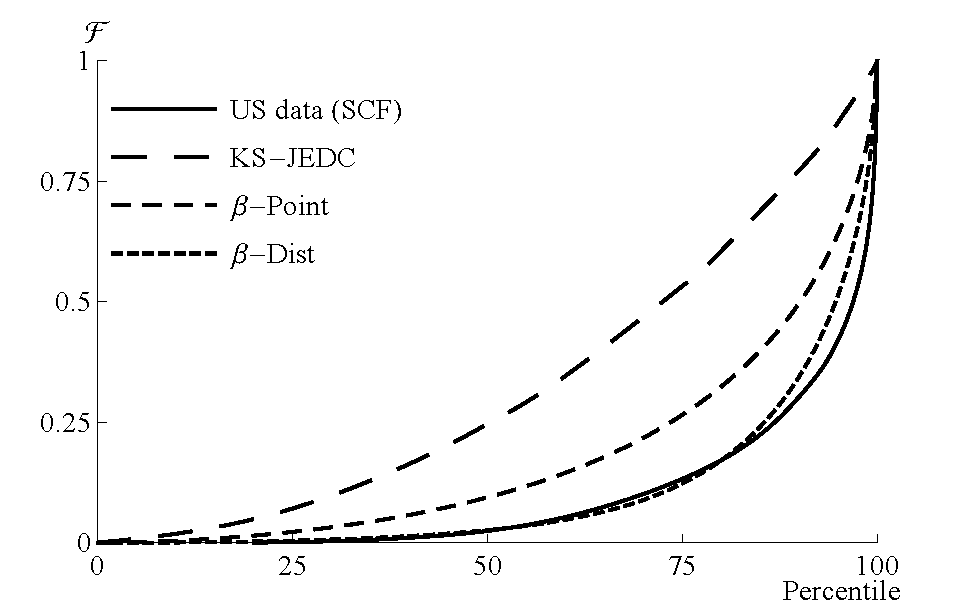
\includegraphics[scale=0.75]{../Figures/LifeCycleLorenzPlot}
\end{center}
\end{figure}

The \Discount-Dist model is able to match the empirical Lorenz curve extremely well for the bottom 85\% of the wealth distribution: the average difference between simulated and actual wealth shares at the levels of interest is less than 0.4\%.  Indeed, the life cycle model is able to match the extremely low asset holdings of the bottom half of the population significantly better than the infinite horizon model.  However, the simulated share of wealth held by the very richest individuals is somewhat lower than the SCF data show; in contrast, the infinite horizon \Discount-Dist model is able to match the Lorenz curve fairly well even in the top 10\%.  We surmise that this is due to differences in the distribution of income at the upper tail between the models.  While about 8\% of households in the infinite horizon model have working lives that exceed 100 years, allowing some of these households to attain extremely high permanent incomes through a series of fortuitous shocks,\footnote{While our results do not critically depend on the inclusion of these very long-lived households, the model requires a somewhat wider distribution of $\Discount$ when they are removed from the aggregation.} individuals in the overlapping generations / finite horizon model retire with certainty after 41 working years, receiving a large negative shock to permanent income and experiencing no income shocks thereafter.  Without the ability to generate extremely high income households, even the richest do not accumulate enough assets to match the top end of the empirical Lorenz curve.  As the simulated distribution matches fairly well and we are concerned with the aggregate marginal propensity to consume, particularly among non-wealthy households, this is not a serious deficiency.


\begin{sidewaystable}
\caption{Average (Aggregate) Marginal Propensity to Consume in Annual Terms, Finite Horizon Life Cycle}
\label{table:MPCallLifeCycle}
\begin{minipage}{\textwidth}
\begin{center}

\begin{tabular}{l c c c c c c c c c}

\toprule
Specification &   \multicolumn{3}{c}{\text{Bequests fully taxed,}}  &  \multicolumn{3}{c}{Bequests distributed,} &  \multicolumn{3}{c}{Bequests distributed,}      \\
&   \multicolumn{3}{c}{\text{no bequest motive}}  &  \multicolumn{3}{c}{no bequest motive} & \multicolumn{3}{c}{with bequest motive} \\
\cmidrule(r){2-4} \cmidrule(r){5-7} \cmidrule(r){8-10}
Model  & \multicolumn{1}{c}{\text{$\Discount$-Point}} & \multicolumn{1}{c}{\text{$\Discount$-Dist}} & \multicolumn{1}{c}{\text{$\Discount$-Dist}} & \multicolumn{1}{c}{\text{$\Discount$-Point}} & \multicolumn{1}{c}{\text{$\Discount$-Dist}}  & \multicolumn{1}{c}{\text{$\Discount$-Dist}} & \multicolumn{1}{c}{\text{$\Discount$-Point}} & \multicolumn{1}{c}{\text{$\Discount$-Dist}} & \multicolumn{1}{c}{\text{$\Discount$-Dist}} \\
\\
Wealth Measure & \multicolumn{1}{c}{Net} & \multicolumn{1}{c}{Net} & \multicolumn{1}{c}{Liquid} & \multicolumn{1}{c}{Net} & \multicolumn{1}{c}{Net} & \multicolumn{1}{c}{Liquid} & \multicolumn{1}{c}{Net} & \multicolumn{1}{c}{Net} & \multicolumn{1}{c}{Liquid} \\
&  \multicolumn{1}{c}{Worth } &  \multicolumn{1}{c}{Worth} &  \multicolumn{1}{c}{Assets} & \multicolumn{1}{c}{Worth} & \multicolumn{1}{c}{Worth} & \multicolumn{1}{c}{Assets} & \multicolumn{1}{c}{Worth} & \multicolumn{1}{c}{Worth} & \multicolumn{1}{c}{Assets} \\
\midrule
Overall average & 0.08  & 0.29 & 0.44 & 0.09 & 0.28 & 0.43 & 0.09 & 0.28 & 0.43 \\
\midrule
By wealth/permanent income ratio  &  & &  & & & & & &  \\
\ Top 1\% & 0.09  & 0.06 & 0.06 & 0.09 & 0.06 & 0.07 & 0.09 & 0.06 & 0.07 \\
\ Top 10\% & 0.08  & 0.07 & 0.06 & 0.09 & 0.07 & 0.07 & 0.09 & 0.07 & 0.07 \\
\ Top 20\% & 0.09  & 0.06 & 0.07 & 0.09 & 0.07 & 0.07 & 0.09 & 0.07 & 0.08 \\
\ Top 30\% & 0.08  & 0.06 & 0.08 & 0.09 & 0.07 & 0.09 & 0.09 & 0.07 & 0.10 \\
\ Top 40\% & 0.08  & 0.07 & 0.12 & 0.08 & 0.08 & 0.13 & 0.08 & 0.08 & 0.14 \\
\ Top 50\% & 0.08  & 0.08 & 0.17 & 0.08 & 0.10 & 0.18 & 0.08 & 0.10 & 0.18 \\
\ Top 60\% & 0.08  & 0.10 & 0.22 & 0.08 & 0.12 & 0.23 & 0.08 & 0.12 & 0.23 \\
\ Bottom 50\% & 0.09  & 0.50 & 0.71 & 0.10 & 0.47 & 0.68 & 0.10 & 0.46 & 0.67 \\
By income  &  & & & & & & & &  \\
\ Top 1\% & 0.07  & 0.24 & 0.38 & 0.08 & 0.29 & 0.42 & 0.08 & 0.29 & 0.42 \\
\ Top 10\% & 0.07  & 0.26 & 0.39 & 0.09 & 0.30 & 0.43 & 0.09 & 0.30 & 0.43 \\
\ Top 20\% & 0.08  & 0.26 & 0.40 & 0.09 & 0.30 & 0.43 & 0.09 & 0.30 & 0.44 \\
\ Top 30\% & 0.08  & 0.27 & 0.40 & 0.09 & 0.30 & 0.43 & 0.09 & 0.30 & 0.44 \\
\ Top 40\% & 0.08  & 0.27 & 0.41 & 0.09 & 0.30 & 0.43 & 0.09 & 0.30 & 0.44 \\
\ Top 50\% & 0.08  & 0.27 & 0.41 & 0.09 & 0.30 & 0.44 & 0.09 & 0.30 & 0.44 \\
\ Top 60\% & 0.08  & 0.27 & 0.41 & 0.09 & 0.30 & 0.44 & 0.09 & 0.30 & 0.44 \\
\ Bottom 50\% & 0.09 & 0.31 & 0.47 & 0.09 & 0.27 & 0.43 & 0.09 & 0.26 & 0.42 \\
By employment status   &  & & & & &  & &  &  \\
\ Employed & 0.08  & 0.29 & 0.43 & 0.09 & 0.28 & 0.42 & 0.09 & 0.27 & 0.42 \\
\ Unemployed & 0.10  & 0.39 & 0.57 & 0.11 & 0.39 & 0.57 & 0.12 & 0.40 & 0.58 \\
\midrule
Time preference parameters   &  & & & & &  & & &  \\
$\grave{\Discount}$   & 0.9911 & 0.9775 & 0.9576 & 0.9899 & 0.9709 & 0.9491 & 0.9898 & 0.9701 & 0.9468 \\
$\nabla$   &  & 0.0391 & 0.0606 &  & 0.0483 & 0.0717 &  & 0.0494 & 0.0748 \\
\bottomrule

\end{tabular}
\end{center}
\footnotesize{Notes: ``Liquid Assets'' refers to liquid financial plus retirement assets, as in the text.
\\The ``with bequest motive'' specification uses bequest parameters of $\alpha = 1$, $\nu = \CRRA$, and $\gamma = 0$.}
\end{minipage}
\end{sidewaystable}

\begin{figure}
\caption{Distribution of MPC's Across Households, Life Cycle Model}
\begin{center}
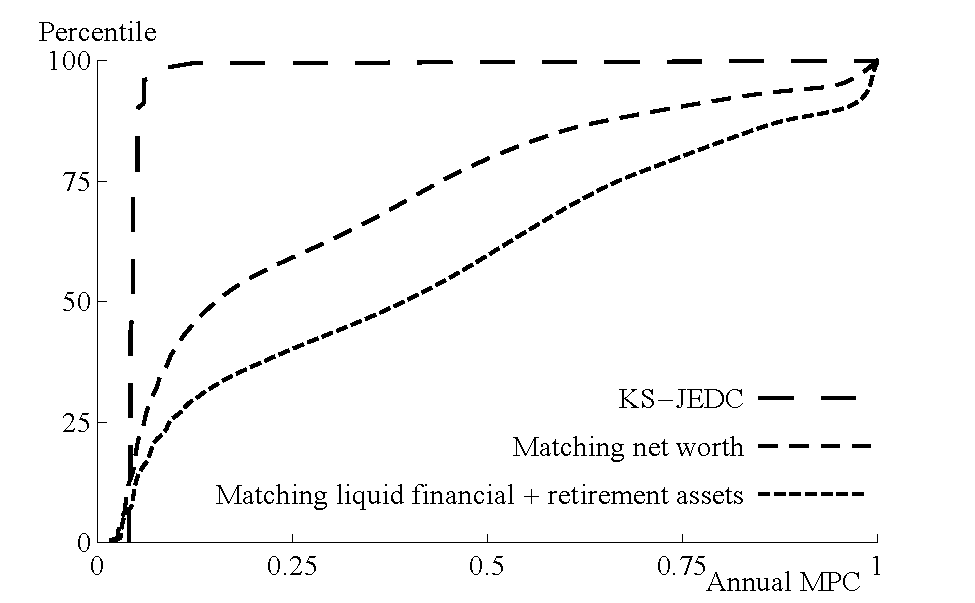
\includegraphics[scale=0.75]{../Figures/MPCdistributionLifeCyclePlot}
\end{center}
\end{figure}

Across all households, the aggregate (annual) marginal propensity to consume in both the \Discount-Point (0.08) and \Discount-Dist (0.29) models is extremely similar to the corresponding averages in the infinite horizon model.\footnote{When the annual marginal propensity to consume is calculated by simulating the change in consumption over four quarters resulting from an unexpected \$1000 payment to each household, we find an aggregate value of 0.28, substantially the same and confirming the same exercise in the infinite horizon model.}  Table \ref{table:MPCallLifeCycle} presents average MPCs for subpopulations.%, parallel to Table \ref{table:MPCall}.
\footnote{Without much comment, we also present estimates of the \Discount-dist model when matching the empirical distribution of liquid financial and retirement assets rather than net worth, along with subpopulation average MPCs for these models.  In each case, the results of the life cycle model align very well with the earlier findings in the infinite horizon setting.}  The relationship between wealth-to-permanent income and the MPC is nearly identical to the pattern in the infinite horizon case, with the MPC slowly rising with lower incomes among the wealthier half of the population, and spiking rapidly among the bottom half.  However, the gradient of income to MPC is much shallower in the finite horizon model, with the wealthiest 1\% of households' MPC only 20\% less than the poorest half, rather than 50\% less in the benchmark model.  This is likely due to confounding effects from life cycle dynamics: income poor households in the overlapping generations model are made up of both the young (who have not had time to accumulate income growth) and the retired (whose cohorts began with lower initial permanent income and have experienced the large negative wage growth from retirement).

While the ratio of wealth to permanent income is a very strong determinant of the marginal propensity to consume in our model, the wide distribution of household incomes allows for even wealthy households to have high MPCs.  Confirming a similar exercise in the benchmark model, we again find that among the one third of households with the highest MPCs, 50\% are in the lowest wealth quintile, 32\% are in the second wealth quintile, and 15\% are in the middle wealth quintile.  Even in a life cycle model in which wealth is highly correlated with both age and the marginal propensity to consume, there is still a significant fraction of ``wealthy hand-to-mouth'' households as found in \cite{kaplanViolanteWeidner_wealthyH2M}.

Figure \ref{fig:MPCbyAge} presents the aggregate marginal propensity to consume by age for the entire population, as well as for the most patient and least patient types in the $\Discount$-Dist model.  After an initial drop as households build up a minimum buffer stock, the life cycle profile of the MPC takes an inverted U-shape for most $\Discount$ types: rising during the rapid income growth ages of 30--50 before falling as households anticipate their retirement and seek to retain assets to consume in old age.  Post retirement, the MPC steadily grows as agents experience an ever increasing mortality risk.  The most impatient households, with a quarterly discount factor of about $\beta = 0.9384$, have a significantly higher MPC throughout life as they disfavor saving---they begin saving for retirement less than ten years prior, and quickly deplete their assets if they live beyond age 75 (as evidenced by MPCs approaching 1 at these ages).  In contrast, the most patient households show an increasing marginal propensity to consume for their entire lives, though beginning from very low levels.

\begin{figure}
\caption{Aggregate Marginal Propensity to Consume by Age}
\label{fig:MPCbyAge}
\begin{center}
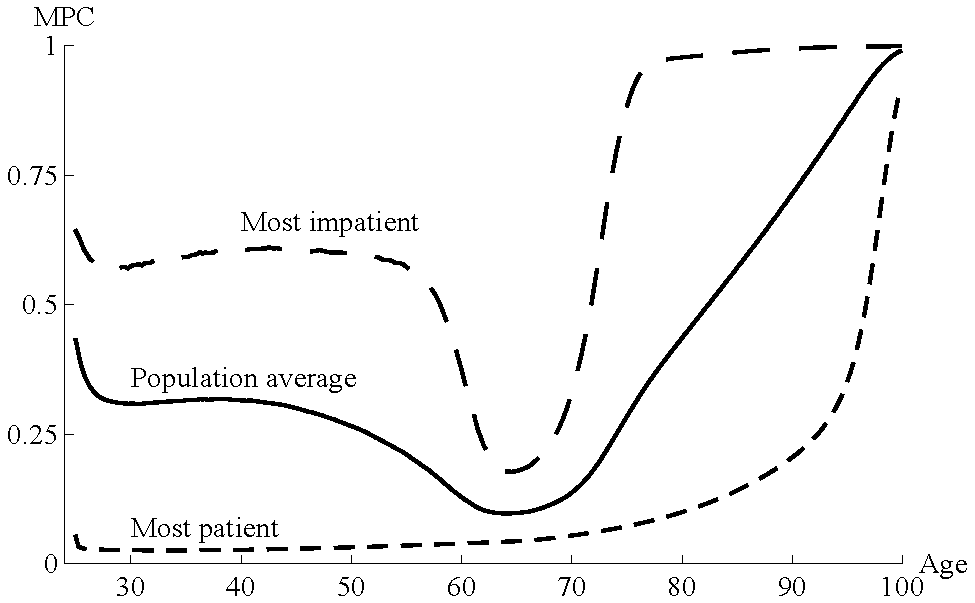
\includegraphics[scale=0.75]{../Figures/MPCbyAgeFigure}
\end{center}
\end{figure}

\subsection{Distribution of Bequests}

The assumption that the assets of the newly deceased are fully taxed away can be relaxed without disturbing our main results.  In the following analyses, we instead assume that these estates are distributed randomly among the population as bequests to other households.  Under a wide range of parameters governing preferences over bequests, both the overall aggregate marginal propensity to consume and its decompositions by wealth and income are little changed from the original specification.

When a household dies at the beginning of time $t$, it receives a one time utility flow\footnote{With apologies to the French, our notation is selected to denote ``grave utility''.} of:
\begin{equation*}
\pLev_t ^{1-\CRRA}\grave{\util}(\kRat_t) = \alpha \frac{(\kRat_t + \gamma)^{1-\nu}}{1 - \nu}.
\end{equation*}
This form combines the approaches of \cite{Cagetti} and \cite{WhyDoRichSave} for maximum flexibility: the factor $\alpha$ controls the absolute magnitude of the bequest motive,\footnote{An individual who is certain to die will have an MPC of approximately $1/(1 + \alpha^{1/\CRRA})$ when $\gamma = 0$ and $\nu = \CRRA$.} the shifter $\gamma$ allows the bequest motive to be completely inactive for lower wealth households, and the curvature parameter $\nu$ determines the extent to which bequests are a luxury good (through the ratio $\CRRA/\nu$).  More complete discussion of the parametrization can be found in the respective sources.  With the bequest motive, the household's consumption Euler equation can be updated to:
\begin{equation*}
\cRat_t^{-\CRRA} = (\daleth +\rProd) \Discount \big( \PLives \Ex_t \left[ (\pshk_{t+1} \cRat_{t+1})^{-\CRRA} \right] + \PDies \alpha(\kRat_{t+1} + \gamma)^{-\nu}\big) \text{ s.t. \eqref{LifeCycleConstraint1}--\eqref{LifeCycleConstraint4}}.
\end{equation*}
The household's problem can be solved by backward induction as before.

As before, the model economy is simulated using a large number of population masses, with each period of a household's life interpreted as the current state of a similar household born in an earlier cohort.  Population masses do not ``die'' during the simulation---they are not discontinued subject to a mortality shock---but rather merely dwindle in population weight as the probability of death accumulates (i.e.\ the mass represents a smaller collection of similar households).  Each age of each simulated mass is assigned a random mass-age (weighting by population mass size) as the beneficiary of bequests given at the end of that period.  If mass $i$ at age $s$ is assigned to bequest to mass $j$ at age $n$, then the ratio of the bequest to mass $j$'s permanent income at age $n$ is:
\begin{equation}\label{eq:Bequest}
b_{is} = \frac{\theta_i \pLev_{i0} \prod_{t = 0}^s (\PLives_{it} \pshk_{it})}{\theta_j \pLev_{j0} \prod_{t = 0}^n (\PLives_{jt} \pshk_{jt})}\big((1 + N)(1 + \Gamma)\big)^{s - n} \kRat_{is}.
\end{equation}
A household might receive multiple bequests at a single age (not uncommon at earlier ages, when population weights are relatively high), or receive none at all.  Bequests are received as a second transitory shock to income, but households do not anticipate this possibility and thus do not account for it in their maximization problem.

As our procedure simulates all population masses simultaneously, the bequest that should be received by a household might be unknown when that age is reached, as it is coming from a population mass at a later age that has not yet been simulated.  To ensure a consistent economy in which the bequests received equal the bequests actually given, we take an iterative approach and estimate the model several times, updating bequests between estimations.  To estimate the extended model, we first set all bequests received to zero and then use the following procedure:\footnote{In practice, simulating the model and updating bequests in steps 2 and 3 is orders of magnitude faster than checking a convergence condition for bequests.  Rather than evaluating a traditional convergence metric, we instead repeat steps 2 and 3 twenty times, more than enough for convergence to occur.  The entire estimation process converges within economically relevant bounds after six applications of step 1, and is thus not overly burdensome.}
\begin{enumerate}
\item Estimate the model assuming the current set of bequests.

\item Using the simulated values of $\kRat_{is}$ at the estimated parameters, update the bequests given by each mass-age using \eqref{eq:Bequest}, then sum bequests received by each mass-age.

\item Simulate the model at the estimated parameters and current set of bequests. Return to step 1 if bequests have not converged to consistent levels.

\item If the new parameter estimates are sufficiently close to the previous estimates (if any), stop; else return to step 1.
\end{enumerate}

We estimate the model at several sets of bequest motive parameters,\footnote{These parameters cannot be meaningfully estimated using our present estimation.  Identification of the three parameters would require matching the distribution of wealth at each age, while we are only concerned with the overall distribution.  The example parameterizations in this section are meant to demonstrate our results' robustness, not as an economic claim.} matching simulated to empirical distributions of both net worth and liquid financial plus retirement assets; the results are reported in additional columns of Table \ref{table:MPCallLifeCycle}.  First, we estimate a specification in which wealth is distributed to survivors, but households attain no utility from providing these bequests: $\alpha$ is set to zero, suppressing the
bequest motive.  Next, we set $\alpha = 1$, $\nu = \rho$, and $\gamma = 0$ as simple choices for a standard bequest motive.  Finally, we test ``extreme'' alternatives by turning the scale of the bequest motive very high ($\alpha = 9$, $\nu = \rho$, $\gamma = 0$) and by specifying bequests as a strong luxury good ($\alpha = 1$, $\nu = \rho/2$, $\gamma = 4$); results of these alternatives are not presented due to space considerations, but are available by request.

As seen in the latter columns of Table \ref{table:MPCallLifeCycle}, the distribution of the marginal propensity to consume in the simulated population is substantially similar whether the assets of the dead are taxed or distributed as bequests, or whether households receive any utility benefit from bequeathed wealth, with only small differences.  Notably, the presence of bequests pushes the estimation to find both a lower median discount factor $\grave{\Discount}$ (0.9775 vs.\ 0.9709 in the case of net worth) and a wider interval $\nabla$ (0.0391 vs.\ 0.0483).  The bottom half of households in the SCF 2004 data hold a very small share of wealth, but in the simulated economy even the poorest households will occasionally receive a substantial bequest.  This tends to boost the share of wealth held by the poorest 20\% and 40\% above the empirical value, requiring the range of $\Discount$ to reach lower for the most impatient households to hold sufficiently low assets to offset this effect.

The variation in average MPC by income is considerably smaller in the presence of bequests, and is almost perfectly flat in some cases.  If a household has received a non-trivial bequest in recent periods, it is less apt to have its consumption habits affected by transitory shocks to income.  More strongly, the random distribution mechanism for bequests greatly weakens the link between income and assets, as income poor households are equally likely to receive large bequests (and when they do, the bequest will be larger relative to their permanent income).  As the household's consumption problem is homothetic in permanent income, this weakened relationship reduces the predictive power of income on the MPC.

We report the results of only the ``simple'' parameters of the bequest motive in Table \ref{table:MPCallLifeCycle}, omitting the more extreme variants.  Just as the distribution of the marginal propensity to consume varies little between the ``no bequest motive'' and ``with bequest motive'' specifications, there is essentially no difference in the MPC as the parameters are shifted about; estimates of the range of discount factors are barely affected.  In short, our key point---that the inclusion of an income process with both permanent and transitory shocks allows a dynamic model to better match microeconomic evidence on the aggregate marginal propensity to consume---relies on neither the infinite horizon assumptions,% of sections \ref{sec:PlausibleAggModel}--\ref{sec:MPC}
the specification of macroeconomic shocks, nor on the particular treatment of bequests.  With a realistic income process and sufficient discount factor heterogeneity to match the empirical distribution of wealth, our results are robust to structural assumptions.

\section{Differences Between $\beta$-Dist and KS-Hetero Models}\label{sec:betaDist}


This section clarifies the channels underlying the differences in MPCs between our preferred model ($\beta$-Dist) and the KS-Hetero model: While in our model the aggregate MPC is quite high, 0.21 (when calibrated to the net worth distribution), in the KS-Hetero model the aggregate MPC is only 0.09.

We address two points:
\begin{enumerate}
\item We analyze in more detail how sensitive the aggregate MPC is to shutting down the permanent ($\psi$) and transitory ($\theta$) income shocks.
\item We investigate the assumption of the uniform distribution we impose on the discount factor $\beta$, and quantify to what extent the assumption drives the results relative to allowing for the permanent--transitory (FBS) income process.
\end{enumerate}

To address these points, we estimated additional specifications, which are summarized in Table~\ref{tAltSpec}. Specifications 1--8 turn off the permanent and transitory income shocks, and the borrowing constraint; specifications  9--12 assume that $\beta$ is log-normally distributed (rather than uniformly).

To preview our results, we find that turning off transitory shocks does not noticeably affect the MPC. Turning off the permanent shocks \emph{and} allowing for borrowing reduces the aggregate MPC from 0.21 to 0.14, each of these two items contributing roughly the same to the decline, compared with the KS-Hetero value of 0.09.  Finally, assuming a log-normal distribution for $\beta$ does not affect the results on MPC much (compared to the baseline, uniform distribution).


\subsection{The FBS Income Process---A Summary }
The FBS household income process \ensuremath{\pmb{y}} includes the permanent component \ensuremath{\pshk} and the transitory shock \ensuremath{\tshk_t}:
\begin{eqnarray}
  \label{eq:tshk}   \label{eq:yLev}
  \yLev_{t} & = & \pRat_{t} \tshk_{t} \Wage_{t}. \notag
\end{eqnarray}
The permanent component follows a geometric random walk:
\begin{eqnarray}
  \label{eq:FBSperm}
  \pRat_{t} & = &  \pRat_{t-1} \pshk_{t},
\end{eqnarray}
where $\pshk$ denotes the white noise permanent shock to income.  The transitory component is:
\begin{eqnarray}
\tshk_{t} &=&\mu \text{ with probability $\mho_{t}$}, \label{eq:unemployed} \\
&=&(1-\tau_{t})\labor\tShkEmp_{t}\text{ with probability $1-\mho_{t}$}, \label{eq:employed}
\end{eqnarray}
where $\mu>0$ is the unemployment insurance payment when unemployed,
$\tau_t$ is the rate of tax collected to
pay unemployment benefits, $\labor$ is time worked per employee and $\tShkEmp_t$ is white noise.

\subsection{Alternative Specifications---Table 1 }

Table~\ref{tAltSpec} considers the implications of switching off the permanent component $\pshk$, the transitory component $\theta$ and of the borrowing constraint:
$$
a_t\ge0.
$$
Specifications 4 and 8 turn off both permanent and transitory income shocks, but keep the unemployment shock $\mho_{t}$ on; this replicates the idiosyncratic income process used in the KS-Hetero model (other than the dependence of $\mho_{t}$ on the macroeconomic state).

\bi
\item Specification 1 is the baseline FBS $\beta$-Dist model reproduced from column 6 of Table~3 in the paper, with the aggregate MPC of 0.21.

\item Specification 2 confirms the referee's point that the MPC has very little sensitivity to shutting down the transitory shock $\theta$.
\item Under specification 3, when the permanent shock is turned off, the aggregate MPC declines to 0.18. The fit of the model worsens, as the Lorenz distance roughly doubles (compared to the baseline).

When transitory and in particular permanent shocks are turned off the width of the band for the discount rate $\nabla$ is smaller. When risk is higher (particularly permanent risk), households want to hold more wealth, so we need to stretch to lower discount factors to get them to hold very little wealth and match the data.  Extra risk has little effect on the wealth holdings of the patient, so the top end of band for $\beta$ does not move.
\item Specification 4 turns off both permanent ($\psi$) and transitory ($\theta$) shocks. The implications are similar to those of specification 3.
\item Specification 5 assumes the baseline FBS income process but allows for borrowing by easing the constraint $a_t\ge0$ to $a_t\ge-2$. Assets are thus allowed to be negative as long as they do not decline below $-2$ times quarterly permanent income, which is the same extent as in the KS-Hetero model. This results in a decline of aggregate MPC from 0.21 to 0.18. The width $\nabla$ reduces somewhat and the fit of the model improves.

\item    Specifications 6, 7 and 8 investigate \emph{the interactions between borrowing and income risk}. If households can borrow, they need to be a bit more patient on the whole to fit the aggregate capital--income target, so they are operating a bit higher on their consumption function, where MPC is lower (specification 5).  In the presence of permanent income risk, a good fraction of them are still on the highly curved portion of the consumption function (which is larger when there is lots of risk), so the MPC is only somewhat lowered. Conversely, when borrowing is not allowed and there is no permanent income risk (specifications 3--4), the consumption function flattens out quickly, but matching the distribution of wealth means some agents are operating very close to the constraint, so even transitory risk is induces precautionary behavior and the MPC again stays relatively high.  When \emph{borrowing is allowed and there is no permanent risk} (specifications 7 and 8), the consumption function becomes flat very quickly and agents are operating above the curved portion, resulting in an appreciably lower MPC.

    The MPC in specification 6 (borrowing and no transitory risk) is essentially the same as in specification 5 (borrowing and transitory risk).
\ei

Specification 8 is closest to the KS-Hetero model both in its structure (simple idiosyncratic income process and with borrowing) and its estimate of the aggregate MPC (0.14 vs 0.09).  The remaining differences between specification 8 and KS-Hetero are the specification of aggregate shocks and the nature of $\beta$ heterogeneity.  As Table 3 in our paper shows that the MPC is similar under the FBS or KS aggregate process (0.21 vs 0.23), we believe the residual difference in MPCs is mostly or entirely accounted for by the vastly different assumptions about the distribution of $\beta$.  Note that the lowest, middle, and highest discrete values of $\beta$ in specification 8 $(0.9869,0.9901,0.9933)$ are \textit{very} close to the three KS $\beta$ values $(0.9858,0.9894,0.9930)$.  However, in specification 8 about 29\% (or 2/7) of simulated agents have an intermediate $\beta$ between the lowest and central types; the corresponding percentiles of $\beta$ in the KS-Hetero model (as well as the 4\% below that) all have $\beta=0.9894$.  As the average MPC is convex in $\beta$, this relative dispersion of the central mass results in an increased MPC in specification 8 relative to KS-Hetero.

To further explore how the structure of $\beta$ heterogeneity affects the aggregate MPC, specifications 9--12 assume that $\beta$ has a \emph{truncated log-normal} distribution (rather than uniform).\footnote{The distribution is approximated with 7 types of households with different $\beta$s.  The discretization of the lognormal distribution was done in the same manner as for the income shock process.} Qualitatively, having a log-normal distribution of $\beta$ generates roughly the same estimated results as a uniform distribution, but with a slightly lower MPC.  The log-normal distribution is more centrally concentrated than the uniform distribution, but not as concentrated as the 10--80--10 assumption in KS-Hetero; thus the average MPC is lower than in the uniform specifications but still higher than KS-Hetero. For specifications 9--11, the log-normal model has a somewhat lower fit in terms of the Lorenz distance than corresponding the uniform models (specifications 1--3), while specification 12 (which allows for borrowing) implies an even better fit than the respective uniform specification (5).

To summarize, turning off the permanent shocks and allowing for borrowing reduces the aggregate MPC from 0.21 to 0.18 each. Both features together reduce the aggregate MPC from 0.21 to 0.14 (compared with the KS-Hetero value of 0.09). Likewise, assuming log-normal $\beta$ also reduces the aggregate MPC by about 0.02.  In contrast, turning off transitory shocks does not noticeably affect the MPC.

\input ../Tables/CSTWaltSpec_bareBones.tex


\nocite{SSLifeTables}

\small
\bibliographystyle{econtex}
\bibliography{economics,cstwMPC,cstwMPC-Add,onlineAppendix_LCM_robustness}


\end{document}



